%%%%%%%%%%%%%%%%%%%%%%%%%%%%%%%%%%%%%%%%%%%%%%%%%%%%%%%%%%%%%%%%%%%%%%
% LaTeX Example: Project Report
%
% Source: http://www.howtotex.com
%
% Feel free to distribute this example, but please keep the referral
% to howtotex.com
% Date: March 2011 
% 
%%%%%%%%%%%%%%%%%%%%%%%%%%%%%%%%%%%%%%%%%%%%%%%%%%%%%%%%%%%%%%%%%%%%%%
% How to use writeLaTeX: 
%
% You edit the source code here on the left, and the preview on the
% right shows you the result within a few seconds.
%
% Bookmark this page and share the URL with your co-authors. They can
% edit at the same time!
%
% You can upload figures, bibliographies, custom classes and
% styles using the files menu.
%
% If you're new to LaTeX, the wikibook is a great place to start:
% http://en.wikibooks.org/wiki/LaTeX
%
%%%%%%%%%%%%%%%%%%%%%%%%%%%%%%%%%%%%%%%%%%%%%%%%%%%%%%%%%%%%%%%%%%%%%%
% Edit the title below to update the display in My Documents
%\title{Project Report}
%
%%% Preamble
\documentclass[paper=a4, fontsize=12pt]{scrartcl}
\usepackage[T1]{fontenc}
\usepackage{fourier}
\usepackage{listings}
\usepackage[english]{babel}		% English language/hyphenation
\usepackage[protrusion=true,expansion=true]{microtype}	
\usepackage{amsmath,amsfonts,amsthm} % Math packages
\usepackage[pdftex]{graphicx}	
\usepackage{url}
\usepackage{graphicx}
\usepackage{float}

%%% Custom sectioning
\usepackage{sectsty}


%%% Custom headers/footers (fancyhdr package)
\usepackage{fancyhdr}
\pagestyle{fancyplain}
\fancyhead{}											% No page header
\fancyfoot[L]{}											% Empty 
\fancyfoot[C]{}											% Empty
\fancyfoot[R]{\thepage}									% Pagenumbering
\renewcommand{\headrulewidth}{0pt}			% Remove header underlines
\renewcommand{\footrulewidth}{0pt}				% Remove footer underlines
\setlength{\headheight}{13.6pt}

%%% Equation and float numbering
\numberwithin{equation}{section}		% Equationnumbering: section.eq#
\numberwithin{figure}{section}			% Figurenumbering: section.fig#
\numberwithin{table}{section}				% Tablenumbering: section.tab#



%%% Maketitle metadata
\newcommand{\horrule}[1]{\rule{\linewidth}{#1}} 	% Horizontal rule

\title{
		%\vspace{-1in} 	
		\usefont{OT1}{bch}{b}{n}
		\horrule{0.5pt} \\[0.4cm]
		\huge Music Recommendation System \\
		\horrule{2pt} \\[0.5cm]
}


%%% Begin document
\begin{document}


\tableofcontents

\pagebreak

\textbf{\large Acknowledgement}
\\
\\
We wish to express our deep gratitude and sincere thanks to Dr. Arun Solanki for his encouragement and for all the facilities that he provided for this project work. We sincerely appreciate this magnanimity by taking us into his fold for which we shall remain indebted to him for his valuable advice and support, which we received from him time to time.
\\
\\
We are thankful to the Dean of ICT Dr Anil Kumar Gautam and all the other faculty and staff members of our department for their kind co-operation and help. Lastly, we would also like to express our deep gratitude towards our seniors and other batchmates for encouraging us throughout the project work.
\pagebreak

\section{Introduction}

Recommender systems typically produce a list of recommendations in one of two ways through collaborative and content-based filtering or the personality-based approach.Collaborative filtering approaches building a model from a user's past behaviour (items previously purchased or selected and/or numerical ratings given to those items) as well as similar decisions made by other users. This model is then used to predict items (or ratings for items) that the user may have an interest in.Content-based filtering approaches utilize a series of discrete characteristics of an item in order to recommend additional items with similar properties.These approaches are often combined (see Hybrid Recommender Systems).
The differences between collaborative and content-based filtering can be demonstrated by comparing two popular music recommender systems Last.fm and Pandora Radio.
Last.fm creates a "station" of recommended songs by observing what bands and individual tracks the user has listened to on a regular basis and comparing those against the listening behavior of other users. Last.fm will play tracks that do not appear in the user's library, but are often played by other users with similar interests. As this approach leverages the behavior of users, it is an example of a collaborative filtering technique.
\\
\\
Pandora uses the properties of a song or artist (a subset of the 400 attributes provided by the Music Genome Project) in order to seed a "station" that plays music with similar properties. User feedback is used to refine the station's results, deemphasizing certain attributes when a user "dislikes" a particular song and emphasizing other attributes when a user "likes" a song. This is an example of a content-based approach.
Each type of system has its own strengths and weaknesses. In the above example, Last.fm requires a large amount of information on a user in order to make accurate recommendations. This is an example of the cold start problem, and is common in collaborative filtering systems.While Pandora needs very little information to get started, it is far more limited in scope (for example, it can only make recommendations that are similar to the original seed).
\\
\\
Two fundamental challenges for collaborative filtering recommender systems.
The first challenge is to improve the scalability of the collaborative filtering algorithms. These algorithms are able to search tens of thousands of potential neighbors in real-time, but the demands of modern systems are to search tens of millions of potential neighbors. Further, existing algorithms have performance problems with individual users for whom the site has large amounts of information.
The second challenge is to improve the quality of the recommendations for the users. Users need recommendations they can trust to help them find items they will like. Users will "vote with their feet" by refusing to use recommender systems that are not consistently accurate for them.In some ways these two challenges are in conflict, since the less time an algorithm spends searching for neighbors, the more scalable it will be, and the worse its quality. For this reason, it is important to treat the two challenges simultaneously so the solutions discovered are both useful and practical.
Recommendations for users are computed by finding items that are similar to other items the user has liked. Because the relationships between items are relatively static,item-based algorithms may be able to provide the same quality as the user-based algorithms with less online computation.

\section{Objective}
Our project has following objectives.
\begin{itemize}	
  \item To implement a Recommendation System using K-Nearest Neighbours Algorithm.
  \item To analyse statistics of proposed system.
  \item To filter the datasets of last.fm.  
\end{itemize}

\section{Prerequisite}
Machine Learning is a field of study that gives computers the ability to learn without being explicitly programmed. Machine learning is closely related to (and often overlaps with) computational statistics, which also focuses in prediction-making through the use of computers. Within the field of data analytics, machine learning is method used to devise complex models and algorithms that lend themselves to prediction; in commercial use, this is known as predictive analytics.
\begin{figure}[H]

\begin{center}

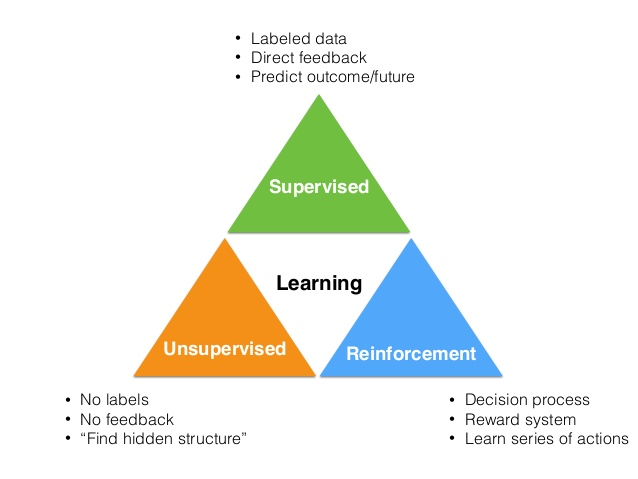
\includegraphics[scale=.4]{ml2.jpg}

 \end{center}

  \caption{Bayes Rule}

  \label{fig:}

\end{figure}
The Figure 3.1 can explained as:- 
\begin{itemize}	
  \item Supervised learning: The computer is presented with example inputs and their desired outputs, given by a "teacher", and the goal is to learn a general rule that maps inputs to outputs
  \item Unsupervised learning: No labels are given to the learning algorithm, leaving it on its own to find structure in its input. Unsupervised learning can be a goal in itself (discovering hidden patterns in data) or a means towards an end (feature learning).
  \item  Reinforcement learning: A computer program interacts with a dynamic environment in which it must perform a certain goal (such as driving a vehicle or playing a game against an opponent). The program is provided feedback in terms of rewards and punishments as it navigates its problem space. 
\end{itemize}

\section{Literature Review}

\textbf{Paper 1: Support-Vector Networks (Vladimir Vapnik 1995)}
\\
\\
SVMs is one of the oldest and most popular algorithms used till date. It works on the idea that input vectors are non-linearly mapped to a very high dimension feature space. In the feature space a linear decision surface is constructed. Special properties of the decision surface ensure high generalization ability of the learning machine. The idea behind the support-vector network was previously implemented for the restricted case where the training data can be separated without errors. Result is extended to non-separable training data. High generalization ability of support-vector networks utilizing polynomial input transformations is demonstrated.
\\
\\
\textbf{Paper 2: A Practical Guide to Support Vector Classification (Chih-wei Hsu , Chih-chung Chang , Chih-jen Lin, 2010)}
\\
\\
The support vector machine (SVM) is a popular classification technique. However, beginners who are not familiar with SVM often get unsatisfactory results since they miss some easy but significant steps. This paper is guide demonstrating a simple procedure which usually gives reasonable results. 
\\
\\
\textbf{Paper 3: Improved support vector machine algorithm for heterogeneous data (Shili Peng, Qinghua Hu, Yinli Chenb, Jianwu Dang, 2015)}
\\
\\
The classical SVM effectively manages classification tasks defined by means of numerical attributes. However, both numerical and nominal attributes are used in practical tasks and the classical SVM does not fully consider the difference between them. Nominal attributes are usually regarded as numerical after coding. This may deteriorate the performance of learning algorithms. With help of this paper, we study a algorithm for learning with heterogeneous data, known as a heterogeneous SVM (HSVM). The proposed algorithm learns a mapping to embed nominal attributes into a real space by minimizing an estimated generalization error, instead of by direct coding.
\\
\\
\textbf{Paper 4: Item-Based Collaborative Filtering Recommendation Algorithms (Badrul Sarwar, George Karypis, Joseph Konstan, and John Riedl, 2001)}
\\
\\
The amount of information in the world is increasing far more quickly than our ability to process it.
Now it is time to create the technologies that can help us sift through all the available information to find that which is most valuable to us. Collaborative filtering works by building a database of preferences for items by users. A new user, Neo, is matched against the database to discover neighbours, which are other users who have historically had similar taste to Neo. Items that the neighbours like are then recommended to Neo, as he will probably also like them. Collaborative filtering has been very successful in both research and practice, and in both information filtering applications and E- commerce applications.
Through this paper, we study issues of recommender systems by applying the approach: item-based algorithms. The bottleneck in conventional collaborative filtering algorithms is the search for neighbors among a large user population of potential neighbors. Item-based algorithms avoid this bottleneck by exploring the relationships between items first, rather than the relationships between users.

\section{Research Methodologies}

The proposed work begins by implementing classification algorithms and then move to K Nearest Neighbors for use in our recommendation system.

\subsection{Naive Bayes}

In machine learning, naive Bayes classifiers are a family of simple probabilistic classifiers based on applying Bayes' theorem with strong (naive) independence assumptions between the features. It remains a popular (baseline) method for text categorization, the problem of judging documents as belonging to one category or the other (such as spam or legitimate, sports or politics, etc.) with word frequencies as the features.The Figure 5.1 describes the Probabilistic model of Naive Bayes
\begin{figure}[H]

\begin{center}

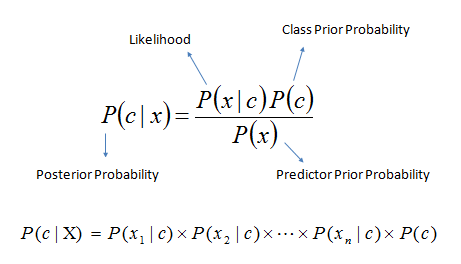
\includegraphics[scale=.4]{Bayes_rule.png}

 \end{center}

  \caption{Bayes Rule}

  \label{fig:}

\end{figure}

Naive Bayes is a simple technique for constructing classifiers: models that assign class labels to problem instances, represented as vectors of feature values, where the class labels are drawn from some finite set. It is not a single algorithm for training such classifiers, but a family of algorithms based on a common principle: all naive Bayes classifiers assume that the value of a particular feature is independent of the value of any other feature, given the class variable. 
An advantage of naive Bayes is that it only requires a small number of training data to estimate the parameters necessary for classification.The figure 5.2
describes how Naive Bayes classifies the data

\begin{figure}[H]

\begin{center}

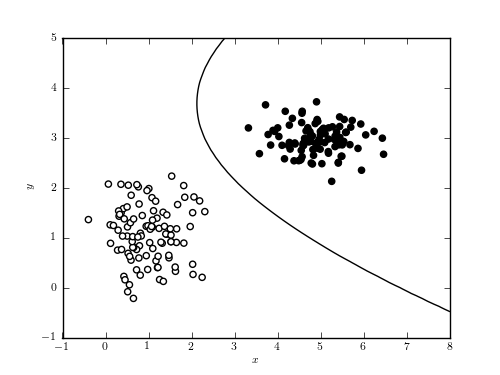
\includegraphics[scale=.6]{nb_scatterplot.png}

 \end{center}

  \caption{Classification using Naive Bayes }

  \label{fig:}

\end{figure}


\subsection{Support Vector Machine}
Support vector machines are supervised learning models with associated learning algorithms that analyze data used for classification Given a set of training examples, each marked as belonging to one or the other of two categories, an SVM training algorithm builds a model that assigns new examples to one category or the other, making it a non-probabilistic binary linear classifier.
Figure 5.3 describes an SVM model which is a representation of the examples as points in space, mapped so that the examples of the separate categories are divided by a clear gap that is as wide as possible. New examples are then mapped into that same space and predicted to belong to a category based on which side of the gap they fall.
\begin{figure}[H]

\begin{center}

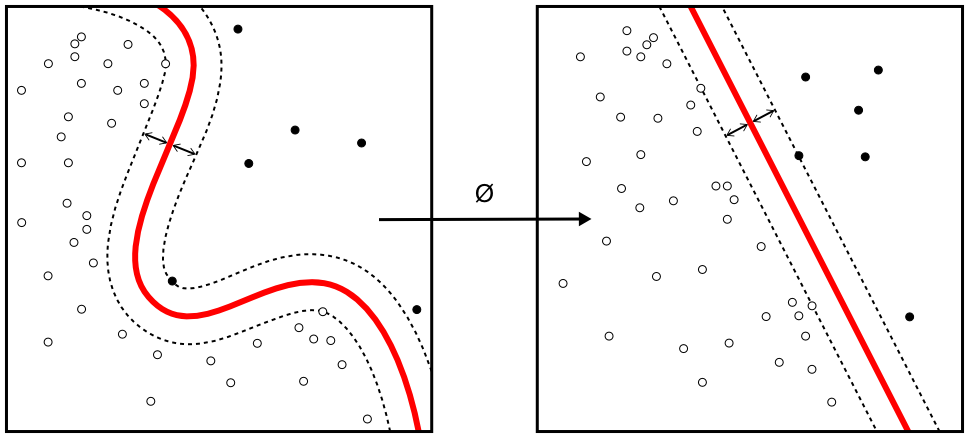
\includegraphics[scale=.6]{svm.png}

 \end{center}

  \caption{Classification using Support Vector Machines}

  \label{fig:}

\end{figure}
In addition to performing linear classification, SVMs can efficiently perform a non-linear classification using what is called the kernel trick, implicitly mapping their inputs into high-dimensional feature spaces. Classifying data is a common task in machine learning. Suppose some given data points each belong to one of two classes, and the goal is to decide which class a new data point will be in. In the case of support vector machines, a data point is viewed as a p-dimensional vector (a list of p numbers), and we want to know whether we can separate such points with a  (p-1) dimensional hyperplane. This is called a linear classifier.
There are many hyperplanes that might classify the data. One reasonable choice as the best hyperplane is the one that represents the largest separation, or margin, between the two classes. So we choose the hyperplane so that the distance from it to the nearest data point on each side is maximized. If such a hyperplane exists, it is known as the maximum-margin hyperplane and the linear classifier it defines is known as a maximum margin classifier.
More formally, a support vector machine constructs a hyperplane or set of hyperplanes in a high- or infinite-dimensional space, which can be used for classification. Intuitively, a good separation is achieved by the hyperplane that has the largest distance to the nearest training-data point of any class (so-called functional margin), since in general the larger the margin the lower the generalization error of the classifier.
\\
SVM Applications
\\
SVMs can be used to solve various real world problems:
\begin{itemize}	
  \item SVMs are helpful in text and hypertext categorization as their application can significantly reduce the need for labeled training instances in both the standard inductive and transductive settings. 
  \item Classification of images can also be performed using SVMs. Experimental results show that SVMs achieve significantly higher search accuracy than traditional query refinement schemes after just three to four rounds of relevance feedback. This is also true of image segmentation systems, including those using a modified version SVM that uses the privileged approach as suggested by Vapnik.
  \item Hand-written characters can be recognized using SVM. 
  \item The SVM algorithm has been widely applied in the biological and other sciences. They have been used to classify proteins with up to 90percent of the compounds classified correctly. Permutation tests based on SVM weights have been suggested as a mechanism for interpretation of SVM models. Support vector machine weights have also been used to interpret SVM models in the past. Posthoc interpretation of support vector machine models in order to identify features used by the model to make predictions is a relatively new area of research with special significance in the biological sciences.
\end{itemize}

\subsection{K-nearest neighbours}
It is a non-parametric method used for classification and regression. In both cases, the input consists of the k closest training examples in the feature space. The output depends on whether k-NN is used for classification or regression:
\\
\\
In k-NN classification, the output is a class membership. An object is classified by a majority vote of its neighbours, with the object being assigned to the class most common among its k nearest neighbours (k is a positive integer, typically small). If k = 1, then the object is simply assigned to the class of that single nearest neighbour.
In k-NN regression, the output is the property value for the object. This value is the average of the values of its k nearest neighbours.
\begin{figure}[H]

\begin{center}

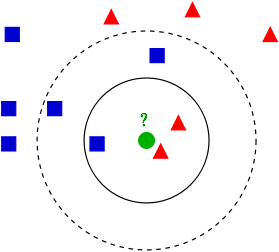
\includegraphics[scale=.6]{knn.png}

 \end{center}

  \caption{Example of k-NN classification}

  \label{fig:}
\end{figure}
The figure 5.4 describes The test sample (green circle) should be classified either to the first class of blue squares or to the second class of red triangles. If k = 3 (solid line circle) it is assigned to the second class because there are 2 triangles and only 1 square inside the inner circle. If k = 5 (dashed line circle) it is assigned to the first class (3 squares vs. 2 triangles inside the outer circle).
\section{Approaches}

\subsection{Collaborative filtering}

One approach to the design of recommender systems that has wide use is collaborative filtering.Collaborative filtering methods are based on collecting and analyzing a large amount of information on users behaviors, activities or preferences and predicting what users will like based on their similarity to other users. A key advantage of the collaborative filtering approach is that it does not rely on machine analyzable content and therefore it is capable of accurately recommending complex items such as movies without requiring an "understanding" of the item itself. Many algorithms have been used in measuring user similarity or item similarity in recommender systems. For example, the k-nearest neighbor (k-NN) approach and the Pearson Correlation as first implemented by Allen.
\\
\\
Collaborative filtering is based on the assumption that people who agreed in the past will agree in the future, and that they will like similar kinds of items as they liked in the past.
\\
\\
When building a model from a user's behavior, a distinction is often made between explicit and implicit forms of data collection.
\\
\\
Examples of explicit data collection include the following:
\\
\\
Asking a user to rate an item on a sliding scale,
Asking a user to search,
Asking a user to rank a collection of items from favorite to least favorite,
Presenting two items to a user and asking him/her to choose the better one of them,
Asking a user to create a list of items that he/she likes.

\subsection{Content-based filtering}
Another common approach when designing recommender systems is content-based filtering. Content-based filtering methods are based on a description of the item and a profile of the users preference.In a content-based recommender system, keywords are used to describe the items and a user profile is built to indicate the type of item this user likes. In other words, these algorithms try to recommend items that are similar to those that a user liked in the past (or is examining in the present). In particular, various candidate items are compared with items previously rated by the user and the best-matching items are recommended. This approach has its roots in information retrieval and information filtering research.
\\
\\
To abstract the features of the items in the system, an item presentation algorithm is applied. A widely used algorithm is the tf idf representation (also called vector space representation).
\\
\\
To create a user profile, the system mostly focuses on two types of information: 1. A model of the user's preference. 2. A history of the user's interaction with the recommender system.
\\
\\
Basically, these methods use an item profile (i.e., a set of discrete attributes and features) characterizing the item within the system. The system creates a content-based profile of users based on a weighted vector of item features. The weights denote the importance of each feature to the user and can be computed from individually rated content vectors using a variety of techniques. Simple approaches use the average values of the rated item vector while other sophisticated methods use machine learning techniques such as Bayesian Classifiers, cluster analysis, decision trees, and artificial neural networks in order to estimate the probability that the user is going to like the item.

\subsection{Hybrid recommender systems}
Recent research has demonstrated that a hybrid approach, combining collaborative filtering and content-based filtering could be more effective in some cases. Hybrid approaches can be implemented in several ways: by making content-based and collaborative-based predictions separately and then combining them; by adding content-based capabilities to a collaborative-based approach (and vice versa); or by unifying the approaches into one model (see for a complete review of recommender systems). Several studies empirically compare the performance of the hybrid with the pure collaborative and content-based methods and demonstrate that the hybrid methods can provide more accurate recommendations than pure approaches. These methods can also be used to overcome some of the common problems in recommender systems such as cold start and the sparsity problem.
\\
\\
Netflix is a good example of the use of hybrid recommender systems. The website makes recommendations by comparing the watching and searching habits of similar users (i.e., collaborative filtering) as well as by offering movies that share characteristics with films that a user has rated highly (content-based filtering).

\pagebreak


\section{Process Model}
\begin{figure}[H]

\begin{center}

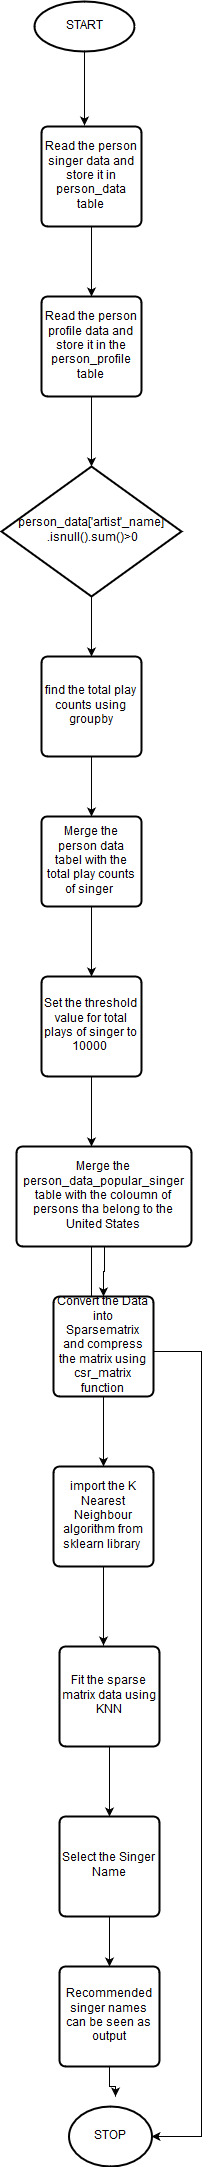
\includegraphics[scale=.7]{process_model.jpg}

 \end{center}

  \caption{Process Model}

  \label{fig:}

\end{figure}

\pagebreak

\section{Pseudo Code}

Step 1 : Import libraries
\\
\\
Step 2 : Read the dataset
\\
\\
Step 3 : Remove the records when artist is NULL
\\
\\
Step 4 : Calculate the total artist plays
\\
\\
Step 5 : Merge the total artist plays with user data
\\
\\
Step 6 : Choose a threshold for popular artists
\\
\\
Step 7 : Filter only popular artists
\\
\\
Step 8 : Reshape the data for implement the Nearest Neighbour Model 
\\
\\
Step 9 : Fit the model
\\
\\
Step 10 : Make the recommendations

\section{Datasets Used}

The Last.fm data are from the Music Technology Group at the Universitat Pompeu Fabra in Barcelona, Spain. The data were scraped by Oscar Celma using the Last.fm API, and they are available free of charge for non-commercial use.
\\
\\	
The Last.fm data are broken into two parts: the activity data and the profile data. The activity data comprises about 360,000 individual users's Last.fm artist listening information. It details how many times a Last.fm user played songs by various artists. The profile data contains each users's country of residence.

\begin{figure}[!b]
  \vspace{1cm}  
  \centering  
  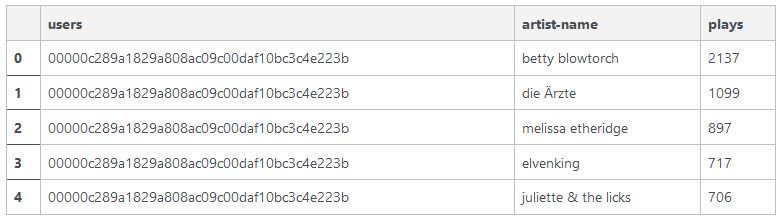
\includegraphics[scale=0.7]{user_data.jpg}
  \caption{user-data}
  \label{fig:boat1}
\end{figure}

	
\begin{figure}[!b]
  \vspace{2cm}
  \centering  
  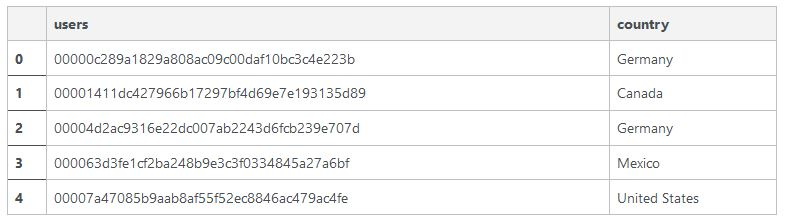
\includegraphics[scale=0.7]{user_profile.jpg}
  \caption{user-profile}
  \label{fig:boat1}
\end{figure}

\section{Libraries Used}
\subsection{Numpy}

NumPy is the fundamental package for scientific computing with Python. It contains among other things:
\begin{itemize}	
  \item a powerful N-dimensional array object
  \item sophisticated (broadcasting) functions
  \item tools for integrating C/C++ and Fortran code
  \item useful linear algebra, Fourier transform, and random number capabilities
\end{itemize}

Besides its obvious scientific uses, NumPy can also be used as an efficient multi-dimensional container of generic data. Arbitrary data-types can be defined. This allows NumPy to seamlessly and speedily integrate with a wide variety of databases. NumPy is licensed under the BSD license, enabling reuse with few restrictions.

\subsection{Pandas}

It is a python data analysis library.
\\
Pandas is an open source, BSD-licensed library providing high-performance, easy-to-use data structures and data analysis tools for the Python programming language.


\subsection{scikit-learn}

Machine Learning library in Python
\begin{itemize}
	\item Simple and efficient tools for data mining and data analysis
	\item Accessible to everybody, and reusable in various contexts
	\item Built on NumPy, SciPy, and matplotlib
	\item Open source, commercially usable - BSD license
\end{itemize}


\section{Result}
Statistics of total artist plays dataset calculated from user data.
\begin{figure}[H]

\begin{center}

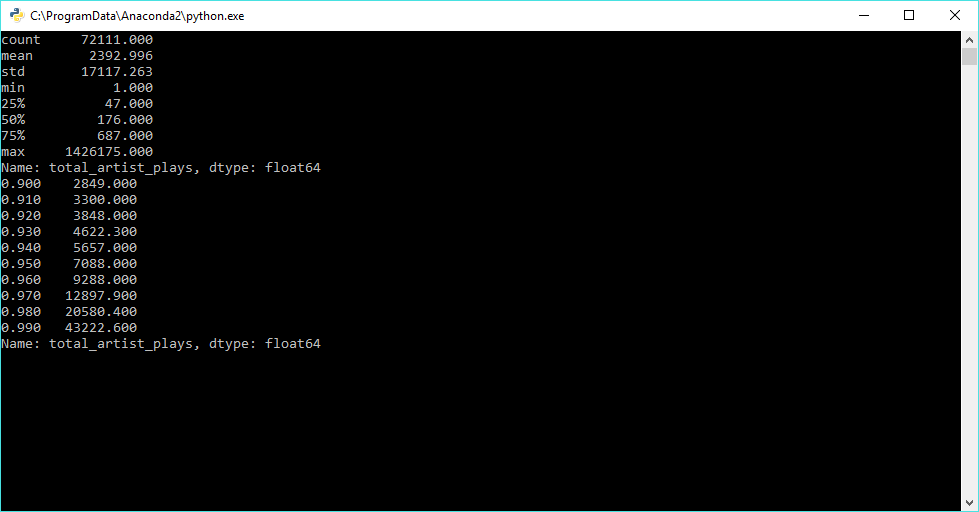
\includegraphics[scale=.6]{result1.png}

 \end{center}

  \caption{Statistics}

  \label{fig:}
\end{figure}  
Graphical User Interface made using TK Engine
\begin{figure}[H]

\begin{center}

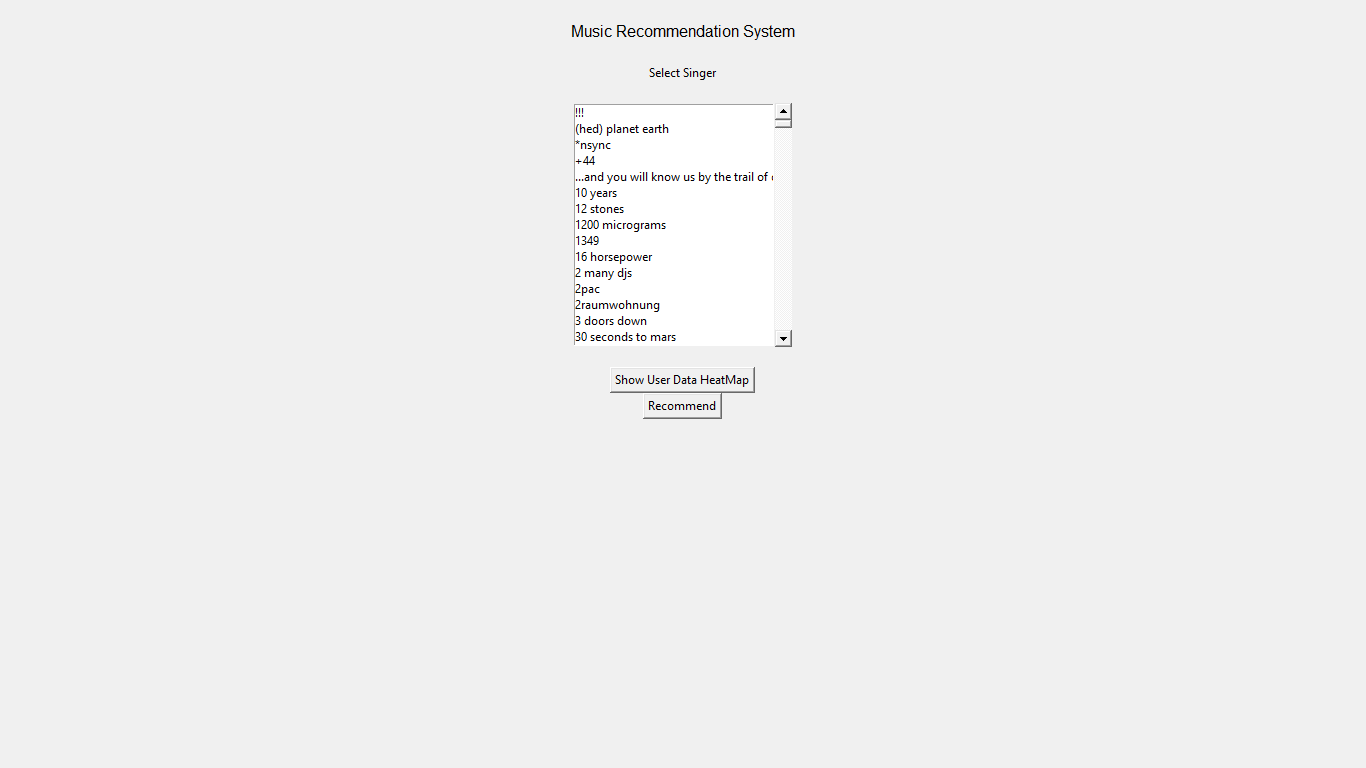
\includegraphics[scale=.4]{gui.png}

 \end{center}

  \caption{Graphical User Interface}

  \label{fig:}
\end{figure}  

\begin{figure}[H]

\begin{center}

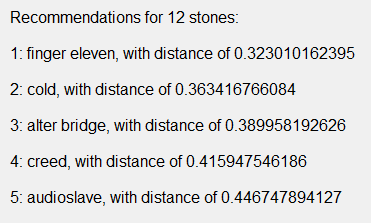
\includegraphics[scale=.8]{recommendations.png}

 \end{center}

  \caption{Recommendations for Selected Artist}

  \label{fig:}
\end{figure} 
 
\begin{figure}[H]

\begin{center}

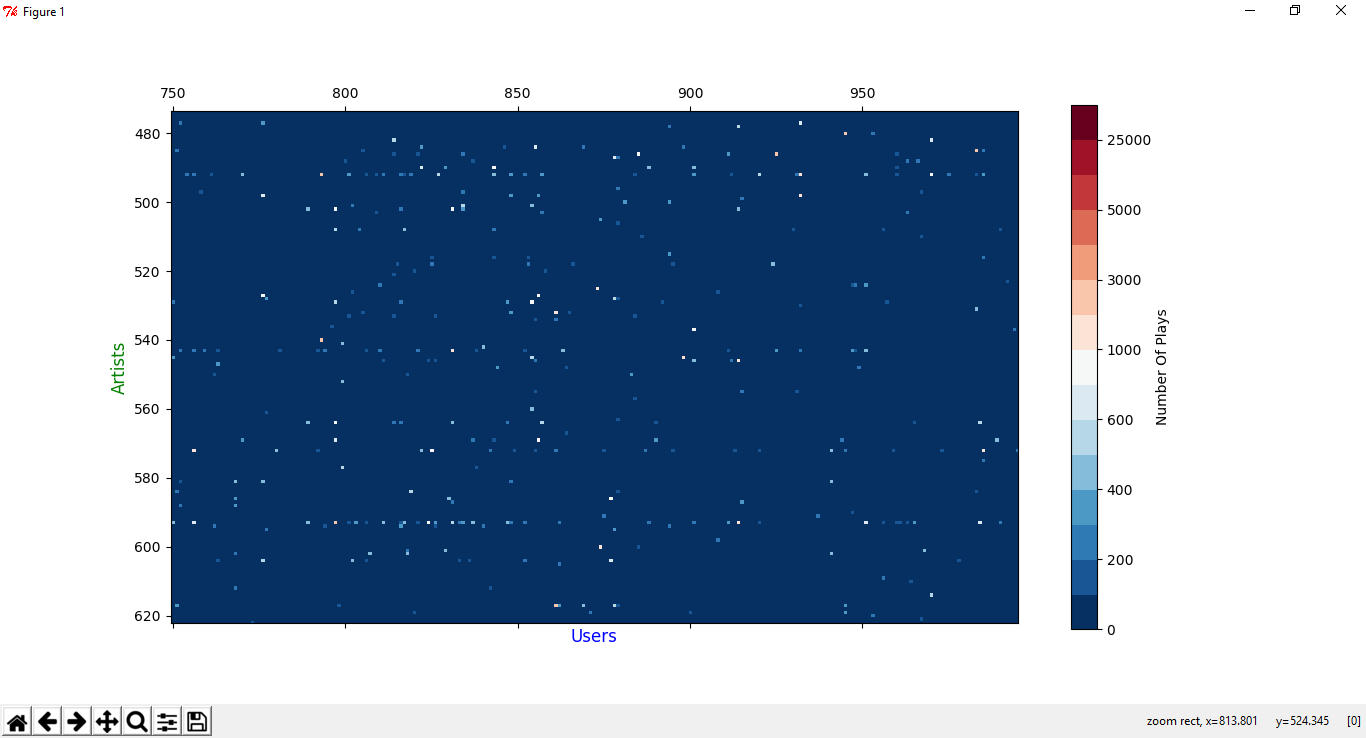
\includegraphics[scale=.5]{graph.png}

 \end{center}

  \caption{HeatMap of Spare Matrix showing number of song plays of artists (Y axis) with respect to users (X Axis).}

  \label{fig:}
\end{figure}  

\pagebreak

\section{Conclusion}

We faced 2 challenges during implementation. 
\\
\\
The first challenge is to improve the scalability of the collaborative filtering algorithm. It algorithm is able to search tens of thousands of potential neighbours in real-time but doesn’t work well with complete dataset. We have efficiently scaled it down by taking filtering only popular artists and then filtered them again according to country such as United States. Next challenge is sparsity. Even active users listened to less than 1% of the artists. With help of sparse matrix, we are able to fill our data with 0s to complete our data. 
\\
\\
This makes our algorithm work well with gigabytes of data we collected from last.fm. Our recommendation system runs successfully

\section{References}

1.	Support-Vector Networks (Vladimir Vapnik, 1995)
\\
\\
2.	Music Recommendations with Collaborative Filtering and Cosine Distance (beckernick.github.io, Nick Becker)
\\
\\
3.	A Practical Guide to Support Vector Classification (Chih-wei Hsu , Chih-chung Chang,  Chihjen Lin, 2010)
\\
\\
4.	Improved support vector machine algorithm for heterogeneous data (Shili Peng, Qinghua Hu, Yinli Chenb, Jianwu Dang, 2015)

\section{Appendix(Code)}


\subsection{UserData.py}
\scriptsize
\begin{lstlisting}

# Import Libraries

import pandas as pd


class User_Data:
	pd.set_option('display.float_format', lambda x: '%.3f' % x)

	# Read Tables

	person_data = pd.read_table('datasets/lastfm-dataset-360K/usersha1-artmbid-artname-plays.tsv',
		                  header = None, nrows = 800000,
		                  names = ['users', 'musicbrainz-artist-id', 'artist-name', 'plays'],
		                  usecols = ['users', 'artist-name', 'plays'])

	person_profiles = pd.read_table('datasets/lastfm-dataset-360K/usersha1-profile.tsv',
		                  header = None,
		                  names = ['users', 'gender', 'age', 'country', 'signup'],
		                  usecols = ['users', 'country'])



\end{lstlisting}


\subsection{PopularArtist.py}
\scriptsize
\begin{lstlisting}

from User_Data import User_Data as ud

class Popular_Artist:
	# Remove Empty Artist Tuples

	if ud.person_data['artist-name'].isnull().sum() > 0:
	    ud.person_data = ud.person_data.dropna(axis = 0, subset = ['artist-name'])

	# Create Artist Table By Grouping Data According to Artist

	singer_plays = (ud.person_data.
	     groupby(by = ['artist-name'])['plays'].
	     sum().
	     reset_index().
	     rename(columns = {'plays': 'total_artist_plays'})
	     [['artist-name', 'total_artist_plays']]
	    )


	person_data_with_singer_plays = ud.person_data.merge(singer_plays, left_on = 'artist-name', right_on = 'artist-name', how = 'left')

\end{lstlisting}

\subsection{Threshold.py}
\scriptsize
\begin{lstlisting}

from Popular_Artist import Popular_Artist as pa
import numpy as np

class Threshold:
	# Analyse data to find threshold

	print pa.singer_plays['total_artist_plays'].describe()
	print pa.singer_plays['total_artist_plays'].quantile(np.arange(.9, 1, .01)), 
	popularity_threshold = 10000

	# Filter populst artist acc to threshold and select United States users

	person_data_popular_singer = pa.person_data_with_singer_plays.query('total_artist_plays >= @popularity_threshold')
	person_data_popular_singer.head()


\end{lstlisting}

\subsection{Country.py}
\scriptsize
\begin{lstlisting}

from Threshold import Threshold as th
from User_Data import User_Data as ud
from scipy.sparse import csr_matrix

class Country:
	combined = th.person_data_popular_singer.merge(ud.person_profiles, left_on = 'users', right_on = 'users', how = 'left')
	usa_data = combined.query('country == \'United States\'')
	usa_data.head()

	# Remove duplicate rows
	if not usa_data[usa_data.duplicated(['users', 'artist-name'])].empty:
	    initial_rows = usa_data.shape[0]

	    print 'Initial dataframe shape {0}'.format(usa_data.shape)
	    usa_data = usa_data.drop_duplicates(['users', 'artist-name'])
	    current_rows = usa_data.shape[0]
	    print 'New dataframe shape {0}'.format(usa_data.shape)
	    print 'Removed {0} rows'.format(initial_rows - current_rows)

	# Convert matrix into sparse matrix
	sparse_singer_data = usa_data.pivot(index = 'artist-name', columns = 'users', values = 'plays').fillna(0)
	sparse_singer_data_compress = csr_matrix(sparse_singer_data.values)


\end{lstlisting}

\subsection{gui.py}
\scriptsize
\begin{lstlisting}

from Tkinter import *

class gui:
	master = Tk()
#	master.attributes('-zoomed', True)
	master.attributes('-fullscreen', True)
	master.title("Music Recommendation System")

	label = Label(master, text="Music Recommendation System", font=7, pady=20)
	label.pack()

	label = Label(master, text="Select Singer")
	label.pack()

	frame = Frame(master, pady=20)
	frame.pack()

	listbox = Listbox(frame, width=33, height=15)
	listbox.pack(side="left", fill="y")

	scrollbar = Scrollbar(frame, orient="vertical")
	scrollbar.config(command=listbox.yview)
	scrollbar.pack(side="right", fill="y")

	listbox.config(yscrollcommand=scrollbar.set)

\end{lstlisting}

\subsection{KNN.py}
\scriptsize
\begin{lstlisting}

from Country import Country as co
import numpy as np
from sklearn.neighbors import NearestNeighbors
from gui import gui as g
from Tkinter import *
import plotHeatMap

# Randomly select artist
#query_index = np.random.choice(co.sparse_singer_data.shape[0])

# Fit filtered data in model
def recommend(algo,dist,inp,query_index):
	
	model_knn = NearestNeighbors(algorithm = algo, metric = dist)
	model_knn.fit(inp)

	# Get nearest neighbours
	distances, indices = model_knn.kneighbors(co.sparse_singer_data.iloc[query_index, :].values.reshape(1, -1), n_neighbors = 6)

	# Display the recommended artists
	abc=''
	for i in range(0, len(distances.flatten())):
	    if i == 0:
		abc += '\n\nRecommendations for {0}:\n\n'.format(co.sparse_singer_data.index[query_index])
	    else:
		if algo=='brute':		
			abc += '{0}: {1}, with distance of {2}\n\n'.format(i, co.sparse_singer_data.index[indices.flatten()[i]], distances.flatten()[i])			
			var.set(abc)
		else:
			#var.set('{0}: {1}, with distance of {2}:'.format(i, wide_artist_data.index[indices.flatten()[i]], 1-(1/(1+distances.flatten()[i])))) 
			var.set(abc)


for item in co.sparse_singer_data.index.values:
    g.listbox.insert(END,item)

frame2 = Frame(g.master, pady=20)
var = StringVar()
label = Message( frame2, textvariable=var, width=500, font="Helvetica 12", pady=-15, padx=20 )
def clickButton():
	if len(g.listbox.curselection())>0 :
		label.config(relief="raised")
		global sel
		sel = g.listbox.curselection()[0]	
		#var.set(str(sel))
		recommend('brute','cosine',co.sparse_singer_data_compress,sel)
		#recommend('kd_tree','euclidean',wide_artist_data,sel)


def showHeatMap():

    mPlotHeatMap = plotHeatMap.plotHeatMap(co.sparse_singer_data);
    mPlotHeatMap.show()


RecommendationButton = Button(g.master, text="Show User Data HeatMap", command=showHeatMap)
RecommendationButton.pack()

b = Button(g.master, text="Recommend", command=clickButton)
b.pack()
label.pack()
frame2.pack()
mainloop()

print '\n'

\end{lstlisting}

\subsection{PlotHeatMap.py}
\scriptsize
\begin{lstlisting}[language=Python]
import matplotlib.pyplot as plt
import matplotlib.colors as colors
import numpy as np
import pandas as pd

class plotHeatMap:
    
    def __init__ (self , sparse_singer_data):
        plt.figure(1)
        plt.switch_backend('TkAgg') #TkAgg (instead Qt4Agg)

        bounds = np.array([0, 100, 200, 300, 400, 500,  600, 700, 1000, 2000, 3000, 4000, 5000, 10000, 25000, 500000]) #MRS intervals
        norm = colors.BoundaryNorm(boundaries=bounds, ncolors=256)

        fig = plt.figure()
        
        ax = fig.add_subplot(111)

        cax = ax.matshow(sparse_singer_data, interpolation='nearest',cmap=plt.get_cmap('RdBu_r'), norm=norm)
        cb = fig.colorbar(cax)
        cb.set_label('Number Of Plays')


#        cax.axes.get_xaxis().set_visible(False)
#        cax.axes.get_yaxis().set_visible(False)

        ax.set_xlabel('Users', fontsize=12, color='Blue')
        ax.set_ylabel('Artists', fontsize=12, color='Green')
        mng = plt.get_current_fig_manager()
        mng.window.state('zoomed')

    def show(self):
        
        plt.show();

\end{lstlisting}
%%% End document
\end{document}